\documentclass[11pt]{article}
\usepackage{geometry}                
\geometry{letterpaper} 
\usepackage{graphicx}
\usepackage{amssymb}
\usepackage{amsmath}
\usepackage{verbatim}
\usepackage{epstopdf}
\usepackage{times}
\usepackage{tikz}
\usetikzlibrary{arrows,automata}
\DeclareGraphicsRule{.tif}{png}{.png}{`convert #1 `dirname #1`/`basename #1 .tif`.png}

\title{CS187 - Homework 2}
\author{Lucas Freitas}
\date{\today}

\begin{document}

\maketitle
\begin {enumerate}

%NUMBER 1
\item
For the purpose of this homework, I decided that a word type should de defined as a sequence of characters such that the first one is a letter from $a$ to $z$ or $A$ to $Z$, and the next ones (if existent), should be characters of any of the following types: word characters (letters, digits, or underscores), apostrophe or hyphen. Using such definition and the following regular expression, we obtained the results shown below.
\\
\\
Regular expression used:
\begin{verbatim}
[a-zA-Z][\w\'\-]*
\end{verbatim}
Output from Python script (available in submission folder as $freitas\_hw2py$):
\begin{verbatim}
Total word tokens in data_part1: 1016737
Total of word types in data_part1: 33436
\end{verbatim}

%NUMBER 2
\item
Output from Python script:
\begin{verbatim}
Total word types that appear only once in data_part1: 14661
\end{verbatim}

%NUMBER  3
\item
Output from Python script:
\begin{verbatim}
Probability the next word is a new word type: 1.4419658181%
\end{verbatim}

%NUMBER 4
\item
For this question and number $8$, I considered that the percentage we are looking for is the percentage of new word types out of all word tokens in both texts combined.
\\
\\
Output from Python script:
\begin{verbatim}
Percentage of new word types in data_part2: 1.35534012937%
\end{verbatim}
From the data above, we can see that the percentage of new word types in $data\_part2$ is $\approx6.007\%$ lower than the Good-Turing estimate from problem $3$.
%NUMBER 5
\item
Output from Python script:
\begin{verbatim}
Total word tokens in data_part1 and data_part2: 2024971
Total of word types in data_part1 and data_part2: 47101
\end{verbatim}

%NUMBER 6
\item
Output from Python script:
\begin{verbatim}
Total number of word types that only appear once in
data_part1 and data_part2: 21136
\end{verbatim}

%NUMBER 7
\item
Output from Python script:
\begin{verbatim}
Probability the next word is a new word type: 1.04376803421%
\end{verbatim}

%NUMBER 8
\item
Using the same assumption from $4$:
\\
\\
Output from Python script:
\begin{verbatim}
Percentage of new word types in data_part3: 1.02496979858%
\end{verbatim}
From the data above, we can see that the percentage of new word types in $data\_part2$ is $\approx1.801\%$ lower than the Good-Turing estimate from problem $7$.

%NUMBER 9
\item
The error of the Good-Turing estimate is clearly lower for number $8$ than for number $4$, which suggests that the Good-Turing method works better for large data sets than for small ones. That implies that if we want to use that method to estimate the number of words in the English language, we should use a very large dataset of words,  which is far from a surprise. If we only used one book to create that estimation, for instance, the Good-Turing estimate would be extremely off, since it would consider that the English language has a number of words somewhat limited to the ones typically used by the author who wrote the book, while if we use a larger dataset, we eliminate that bias and augment our "English vocabulary", leading to a better estimate. 

%NUMBER 10
\item
Zipf's equation states that:
$$r\cdot f(t_r)=K$$
Taking the logarithm of both sides:
$$log(r)+log( f(t_r))=log(K)$$
$$log( f(t_r))=-log(r)+log(K)$$
That just means that in logarithmic scale, the graph of frequency versus rank will be a straight line, so we just need to take the empirical data we obtained and find the line that best fits those points.
\\
\\
The graph obtained is:
\begin{center}
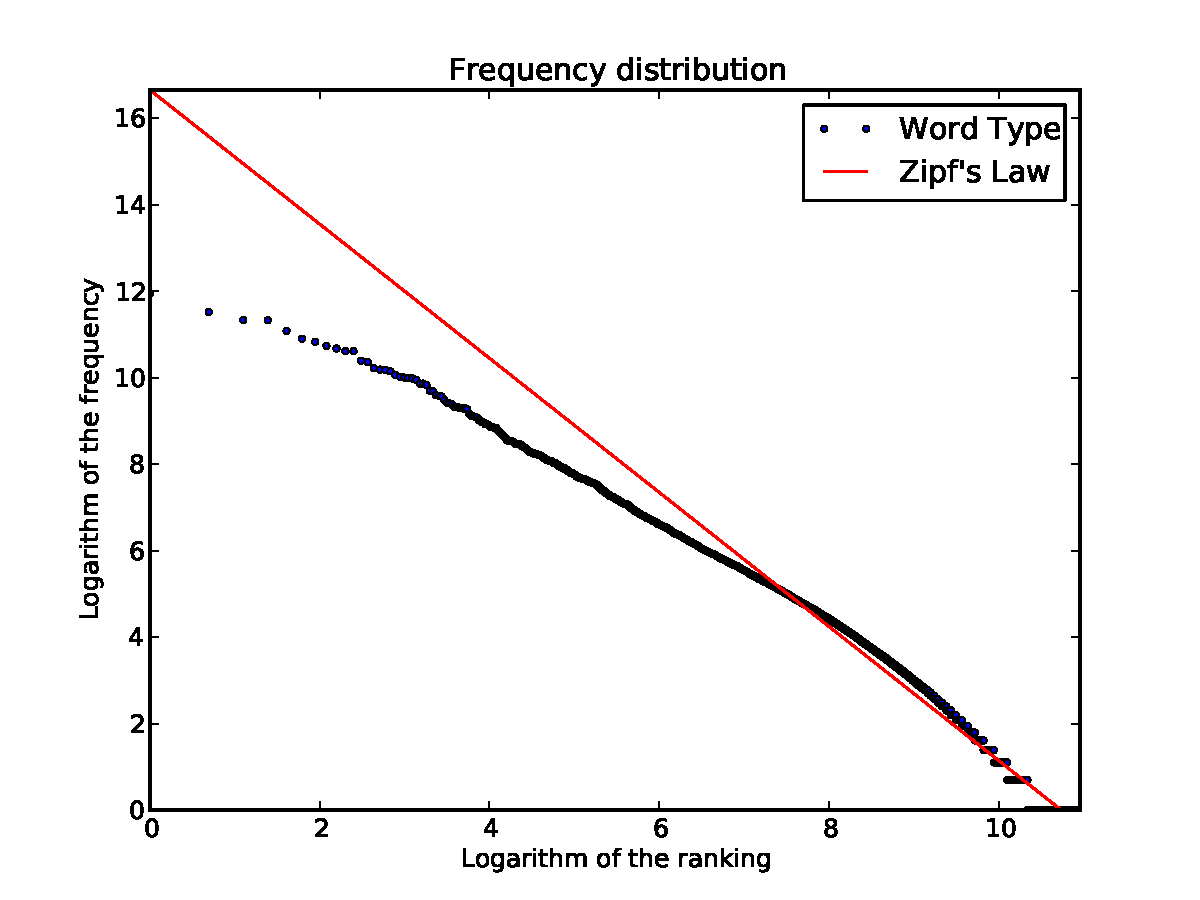
\includegraphics[width=140mm]{graph.pdf}
\end{center}

Notice that the line gets closer to the points on the right, since the density of points in that area is exponentially larger than the density on the left.
%NUMBER 11
\item
The corpus seems to follow Zipf's equation for intermediate rank values. If the rank is too low, the frequency is extremely noisy, since large frequency values are rather rare, and not uniformly distributed at all. As the rank increases, however, both rank and frequencies are more uniformly distributed and the corpus follows Zipf's equation with very small error. For extremely large rank values, however, the number of word types in which the frequency is the same is very large, and the corpus stops following Zipf's equation once again. That way, Zipf's law is pretty effective for intermediate rank values, but a perfect line cannot be obtained including all points in the curve.

\end{enumerate}
\end{document}  